\section{The Problem}\label{the-problem-2}

\subsection{Plate Theory}\label{plate-theory}

\subsection{Boundary Conditions}\label{boundary-conditions}

\section{The Solution}\label{the-solution-1}

\subsection{Implementation}\label{implementation}

\subsubsection{Discretising}\label{discretising}
\subsubsection{Design}\label{design}

\section{Application}\label{application-1}

\section{INTRODUCTION}
\noindent
Plate vibration is a longstanding topic of research. Plates are common engineering elements finding application in industry and, particularly, in acoustics. Musical instrument soundboards are accurately described using appropriate plate theories such as Kirchhoff-Love \cite{love_small_1888} and Mindlin-Reissner \cite{mindlin_Influence_1951}. Furthermore, plates lend themselves naturally to understanding vibration through eigenshape visualisation. They are often used as teaching tools in classrooms for their ability to produce accurate and fascinating Chladni patterns \cite{chladni_treatise_nodate}. Eigenshape visualisation techniques are still used today to measure the elastic properties of tonewood \cite{ducceschi_method_2024,fletcher_physics_2012} parallel to numerical simulation. Despite such an ever-growing body of applications, plate simulation is still mostly accessible through dedicated, proprietary software, often out of reach for the typical student's budget or even for small-sized research groups. This work illustrates the theoretical foundation and a first implementation of MAGPIE. MAGPIE is designed to be an open-source platform to simulate the physics of plates, offering easy-to-use visualisation tools and several analysis techniques. The tools can be equally used as a teaching aid for lecturers and as an analysis tool for researchers and industry stakeholders. Functionalities include setting elastic boundary conditions along the plate edges, visualising eigenshapes, exporting eigenshapes and frequencies, performing a time-domain simulation of the plate equation for sound synthesis, and estimating the elastic modulus of experimental plates. For brevity, not all functionalities can be described in this work, and attention is here restricted to the eigenvalue problem and related implementation. In Section \ref{sec:BackGround}, the background plate physics is described, along with the numerical approach used to perform the simulations; in Section \ref{sec:implementation}, the implementation details of MAGPIE are discussed; finally, Section \ref{sec:Conclusions} draws some final reflections and illustrates future alleys of development. 


\section{Theoretical Background}\label{sec:BackGround}
\noindent
The Kirchhoff-Love theory of plates describes the dynamics of thin sheet materials under bending. Assuming constant thickness and density, and with the further hypothesis of isotropy, a linear partial differential equation describing wave propagation is, thus \cite{graff1991wave,bilbao_numerical_2009}:
\begin{equation}\label{eq:KLCnt}
\rho \zeta \frac{\partial^2 u}{\partial t^2} = - D \Delta\Delta u - 2\rho\zeta\sigma\frac{\partial u}{\partial t} + \delta(x-x_p)\delta(y-y_p)f(t).
\end{equation}
In the above, $u = u(x,y,t) \in {\mathcal D} \times \mathbb{R}^+_0 \rightarrow \mathbb{R}$ is the flexural displacement of the plate, occupying a rectangular domain ${\mathcal D} := [0,L_x] \times [0,L_y]$, where $L_x$, $L_y$ are the side lengths along the $x$ and $y$ axes, respectively. In the above, constants appear as: $\rho$, the volume density of the plate (in kg $\cdot$ m$^{-3}$); $\zeta$, the plate thickness, assumed uniform throughout ${\mathcal D}$ (in m); $D := E\zeta^3 / 12 (1-\nu^2)$, the rigidity of the plate, where $E$ is Young's modulus (in Pa), and $\nu$ is Poisson's ratio. In the equation, $\Delta$ represents the two-dimensional Laplace operator:
\begin{equation}
\Delta := \frac{\partial^2}{\partial x^2} + \frac{\partial^2}{\partial y^2},
\end{equation}
$\Delta\Delta$ is, thus, the two-dimensional biharmonic operator. $\sigma$, measured in s$^{-1}$, is a loss factor. $f(t)$ is an external input, and $(x_p,y_p)$ is the input location on the plate surface. The input is distributed according to a double Dirac delta and is, hence, pointwise.

\eqref{eq:KLCnt} may be arrived at after inspection of the energy of a bent plate. To that end, consider the definitions of inner product and associated norm for two smooth functions defined over $\mathcal{D}$:
\begin{equation}
\innp{f,g} := \int_{\mathcal D} f\,g\,\mathrm{d}x\mathrm{d}y, \quad \norm{f} = \sqrt{\innp{f,f}}.
\end{equation}
Furthermore, consider the following bilinear operator:
\begin{equation}\
\mathcal{L}(f,g) := \frac{\partial^2 f}{\partial x^2}\frac{\partial^2 g}{\partial y^2} + \frac{\partial^2 f}{\partial y^2}\frac{\partial^2 g}{\partial x^2} - 2\frac{\partial^2 f}{\partial x\partial y}\frac{\partial^2 g}{\partial x\partial y}.
\end{equation}
With this notation, the form of the energy can be expressed compactly as:
\begin{equation}\label{eq:CntEn}
\mathfrak{H} := \frac{\rho}{2}\norm{\frac{\partial u}{\partial t}}^2 + \frac{D}{2}\left(\norm{\Delta u}^2 + (\nu-1)\innp{\mathcal{L}(u,u),1}\right),
\end{equation}
and the energy balance reads:
\begin{equation}\label{eq:EnBalCnt}
\frac{d \mathfrak{H}}{dt} = -2\rho\zeta\sigma\norm{ \frac{\partial u}{\partial t}}^2 + \frac{\partial u}{\partial t}(x_p,y_p,t)f(t).
\end{equation}
In particular, energy is conserved in the absence of dissipation ($\sigma = 0$) and external forcing ($f=0$).
The form of the energy is more complicated than what one would expect after a cursory examination of \eqref{eq:KLCnt}. In fact, one may have trouble bounding the energy from below by just glancing at the form of the energy, as the inner product involving the bilinear operator $\mathcal L$ is not, by definition, non-negative. Bilbao \cite[Chapter 11]{bilbao_numerical_2009} noted that the inner product involving the operator $\mathcal L$ in the energy expression only contributes to boundary terms, and it does not change the energy in the domain interior, as one may show after integrating by parts the inner product in the energy expression. See also \cite{thomas2008geometrically}. The boundary terms appear as the energy-conjugate products force/velocity and moment/angular velocity. For a side perpendicular to the $x$ axis, the analytic expressions for the force and moment are derived as:
\begin{equation}
\mathfrak{F}_x := D \left(\frac{\partial^3 u}{\partial x^3} + (2-\nu)\frac{\partial^3 u}{\partial x \partial y^2}\right), \quad \mathfrak{M}_x := -D\left(\frac{\partial^2 u}{\partial x^2} + \nu \frac{\partial^2 u}{\partial y^2} \right).
\end{equation}
The boundary terms along the edges located at $x=0,L_x$ are, thus:
\begin{equation}
    \mathfrak{B}_{x=L_x}= \int_{0}^{L_y}\left(\frac{\partial u}{\partial t}\mathfrak{F}_x + \frac{\partial^2 u}{\partial t\partial x}\mathfrak{M}_x\right)\,\mathrm{d}y\,\Big|_{x=L_x}\,,\quad
    \mathfrak{B}_{x=0}= -\int_{0}^{L_y}\left(\frac{\partial u}{\partial t}\mathfrak{F}_x + \frac{\partial^2 u}{\partial t\partial x}\mathfrak{M}_x\right)\,\mathrm{d}y\,\Big|_{x=0}\,.
\end{equation}
The boundary terms for the edges at $y = 0,L_y$ are obtained using analogous expressions for the force and moment ${\mathfrak F}_y$, ${\mathfrak M}_y$: one only needs to swap $x$ and $y$ in the expressions for ${\mathfrak F}_x$, ${\mathfrak M}_x$. With these in mind, one can easily recover the expressions for free, clamped and simply supported edge conditions: in the free case, the force and the moment vanish; in the clamped case, the displacement and the slope vanish; in the simply supported case, the displacement and the moment vanish. For all such cases, the boundary terms vanish, so the total plate energy follows the energy balance above. One further condition arises at the corner of two free edges, namely:
\begin{equation}\label{eq:CornerCnt}
\frac{\partial^2 u}{\partial x \partial y} = 0,
\end{equation}
see, for example, the book by Szilard for an explanation \cite{szilardBook}.


\subsection{Elastically restrained plates}

The boundary conditions of the classic type form a set of consistent conditions leading to the energy balance expressed in \eqref{eq:EnBalCnt}. In some cases, the edges can themselves store energy, such as when the plate is elastically restrained. This case has received some attention in previous literature, particularly in Galerkin-type applications; see, for example, \cite{li2009exact,zhang2009vibrations,li2000free}. One reason for such interest lies in the ability to recover the classic edge conditions for limiting values of the edge stiffness constants. When a plate is elastically restrained, two spring-like devices control the displacement and the rotation of the edge by delivering counteracting elastic force and moment. At the simulation level, one can observe the passage from one end condition to another by varying the stiffness of one or more springs along the edges. This leads to modal crossings, including distortion of the modal shapes, which may be a useful analysis tool in various scenarios, particularly in modal-based vibration analysis. The boundary conditions of an elastically restrained plate along $x=L_x$ and $x=0$ are as follows:
\begin{subequations}
\begin{align}
K_{xL_x} u(L_x,y,t) &= {\mathfrak F}_x(L_x,y,t), \quad R_{xL_x} \frac{\partial u}{\partial x}(L_x,y,t) = {\mathfrak M}_x(L_x,y,t); \\
K_{x0} u(0,y,t) &= -{\mathfrak F}_x(0,y,t), \quad R_{x0} \frac{\partial u}{\partial x}(0,y,t) = -{\mathfrak M}_x(0,y,t).\label{eq:BCsCnt2}
\end{align}
\end{subequations}
Here, $K_\circ$, $R_{\circ}$ denote the flexural and rotational spring stiffness constants, respectively. Remark that the units of $K_\circ$ are N $\cdot$ m$^{-2}$, as the boundary force $F_\circ$ is per unit length. Similarly, $R_{\circ}$ is measured in N $\cdot$ m$^{-1}$.
The expressions for the boundary conditions at the edges along $y=0,L_y$ can be given analogously. Note that the boundary force vanishes whenever $K_\circ$ vanishes. Conversely, the displacement vanishes as $K_\circ \rightarrow \infty$. The moment vanishes whenever $R_{\circ}$ vanishes and the slope vanishes whenever $R_\circ \rightarrow \infty$. Note that the presence of the elastic edge supports modifies the expression of the energy. Thus, \eqref{eq:CntEn} is not the overall energy of the bent plate. The complete expression is here omitted for brevity but is available in \cite{szilardBook}, depending on eight elastic constants (i.e. four flexural spring constants $K_\circ$ and four rotational spring constants $R_\circ$).

\subsection{Semi-discrete equations}

The method of finite differences can be employed to simulate \eqref{eq:KLCnt}. To that end, space is first discredited using a grid of points with equal spacing along $x$ and $y$. Let $h$ be such grid spacing. Thus, the domain $\mathcal D$ is sampled with a two-dimensional grid of size $M:=(M_x+1)(M_y+1)$, with $M_x$ being the number of grid subintervals along $x$, and $M_y$ being the number of grid subintervals along $y$. The continuous displacement $u(x,y,t)$ is thus approximated by a two-dimensional grid function $u_{l,m}$, which may itself be turned into a column vector ${\bf u}(t)$ of length $M$. Turning the two-dimensional grid function into a column vector can be achieved as in Figure \ref{fig:PlateFD}, by stacking consecutive strips of grid points sharing the same index $l$.
\begin{figure}
\centering
\includegraphics[width=0.9\linewidth]{img/plateGrid.pdf}
\caption{Sketch of the finite difference method discretising the plate equation. On the left, the 13-point biharmonic coefficients are scaled by $h^{-4}$\cite{tee_novel_1963}.}\label{fig:PlateFD}
\end{figure}
Approximating derivatives is easily accomplished via the following definitions of the difference operators:
\begin{subequations}
\begin{align}
\dsd u_{l,m} := (2h)^{-1}\left(u_{{l+1},m} - u_{{l-1},m} \right) \approx \partial u / \partial x, \\ 
\dss u_{l,m} := h^{-2}\left(u_{{l+1},m} - 2u_{l,m} + u_{{l-1},m} \right) \approx \partial^2 u / \partial x^2,\\ 
\dssss u_{l,m} := \dss (\dss u_{l,m}) \approx \partial^4 u / \partial x^4,
\end{align}
\end{subequations}
with similar definitions holding for the derivatives along $y$. Thus, a discretisation of the biharmonic operator is obtained as:
\begin{equation}
\Delta\Delta \approx \dssss + \delta_{yyyy} + 2\dss\delta_{yy}.
\end{equation}
When applied to a grid point away from the boundary, the resulting 13-point biharmonic difference operator has coefficients as per Figure \ref{fig:PlateFD}. Closer to the boundary, the coefficients must be specialised to account for the boundary conditions. A discretisation of, e.g. \eqref{eq:BCsCnt2} is given here as:
\begin{equation}
K_{x0}u_{0,m}=-D(\dss + (2-\nu)\delta_{yy})\dsd u_{0,m}, \quad R_{x0}\dsd u_{0,m} = D(\dss + \nu\delta_{yy})u_{0,m}.
\end{equation}
Analogous conditions can be given at the other edges. The corner condition \eqref{eq:CornerCnt} may be discredited at the upper-left corner as:
\begin{equation}\label{eq:CornerFD}
\delta_{x\cdot}\delta_{y\cdot} u_{0,0} = 0,
\end{equation}
and similarly at the other three corners. 
\begin{figure}
\centering
\includegraphics[width=0.4\linewidth]{img/plateBCs1.pdf}
\caption{Ghost points resulting from applying the biharmonic difference operator to the upper-left corner.}\label{fig:PlateGhostFD}
\end{figure} 
Figure \ref{fig:PlateGhostFD} shows the seven ``ghost'' points resulting from applying the biharmonic operator to $u_{0,0}$. Such seven values are set by applying the moment boundary condition to $u_{0,1}$ and $u_{1,0}$, plus the moment and force conditions along $x$ and $y$ to $u_{0,0}$. These are six conditions in total. The seventh condition is given by \eqref{eq:CornerFD}. The resulting biharmonic coefficients have extremely lengthy expressions, omitted here for brevity, but presented on the GitHub page of MAGPIE \cite{MAGPIE_project_url}. However, the resulting biharmonic matrix is sparse, with a sparsity pattern as per Figure \ref{fig:PlateGhostFD}.


\subsection{Eigenvalue problem and time stepping scheme}

Let $\bf B$ denote the resulting biharmonic matrix of size $M \times M$. $\bf B$ is generally not symmetric, but it possesses a set of $M$ independent, real eigenvectors for sufficiently small $h$. The eigenvalues are also real and bounded from below. For a completely free plate, the eigenvalues are found in the range
\begin{equation}\label{eq:EigenBounds}
0  \lessapprox \lambda_{\bf B} \leq 64 h^{-4},
\end{equation}
where the approximate left inequality is due to the rigid-body eigenvalues becoming negative in a very small neighbourhood around zero. For elastically restrained plates, the eigenvalues are bounded according to:
\begin{equation}
0 \lessapprox \lambda_{\bf B} \leq \mathcal{O}(\text{max}(R_\circ,K_\circ)), 
\end{equation}
where the ``big-Oh'' notation was used. Thus, when the plate is restrained using very stiff springs, the spectral radius of the matrix becomes large. Whilst most of the eigenvalues will still be found within the bounds in \eqref{eq:EigenBounds}, a handful of ``spurious'' eigenvalues and associated modal shapes may result from applying the elastic boundary conditions using very large stiffness constants. In any case, the matrix $\bf B$ is factorised according to:
\begin{equation}\label{eq:factorisation}
{\bf B} = {\bf Q}{\boldsymbol \Lambda}{\bf Q}^{-1},
\end{equation}
where ${\boldsymbol \Lambda}$ is a diagonal matrix of eigenvalues, and $\bf Q$ is a matrix of associated column eigenvectors. The plate eigenfrequencies, in radians per second, are obtained as:
\begin{equation}
{\boldsymbol \Omega} = \sqrt{\frac{D}{\rho\zeta}} \sqrt{{\boldsymbol \Lambda}},
\end{equation}
where taking the square root of the eigenvalues is justified according to the bounds above. A semi-discrete version of \eqref{eq:KLCnt} results as:
\begin{equation}\label{eq:SemiDisc1}
\rho \zeta \ddot {\bf u}(t) = -D{\bf B}{\bf u}(t) - 2\rho\zeta\sigma\dot {\bf u}(t) + h^{-2}{\bf J} f(t).
\end{equation}
Note that overdots now denote total time derivates. In the above, $\bf J$ is a sparse vector discretising the double Dirac delta. Many options are available, such as via Lagrange interpolants, see \cite{bilbao_numerical_2009}. Using the factorisation \eqref{eq:factorisation}, diving both sides of \eqref{eq:SemiDisc1} by $\rho \zeta$ and multiplying both sides by ${\bf Q}^{-1}$, the following system results:
\begin{equation}\label{eq:ModalSyst}
\ddot {\bf w}(t) = -{\boldsymbol \Omega}^2 {\bf w}(t) -2 {\bf C}\dot {\bf w}(t) + \rho^{-1}\zeta^{-1}h^{-2}{\bf Q}^{-1}{\bf J}f(t),
\end{equation}
where ${\bf w}(t) := {\bf Q}^{-1}{\bf u}(t)$. This is a completely parallel (i.e. diagonal) system of $M$ lossy, forced oscillators, with natural frequency $\Omega_m$, $1\leq m\leq M$. Note that the loss matrix $\bf C$ can now contain different loss factors $\sigma_m$ for different modes, such as from experimental measurements.  


One can truncate the system to an integer $N < M$, and work with the modes belonging to a given frequency band. One may, for instance, solve the eigenvalue problem \eqref{eq:SemiDisc1} using a very fine grid for increased precision but only retain the modes for which the natural frequency falls within the audible range. System \ref{eq:ModalSyst} may then be updated in time using the ``exact'' integrator for the lossy oscillator, see e.g. \cite{Cieśliński_JDEA_2011} thus, yielding numerical simulations with very low numerical dispersion.


\section{IMPLEMENTATION}\label{sec:implementation}

MAGPIE collects together functionality for computing a discrete biharmonic operator, eigensolver, and impulse response generation through modal time integration and Young's modulus estimation. As discussed previously, the full extent of the functionality cannot be fully covered in this paper. This section aims to cover the main development steps and choices taken during the development of MAGPIE, technical underpinnings, justification and a case study of a hypothetical library application.

\noindent
MAGPIE was originally planned as a library for Python, as it is a free open-source platform. During the development, it became apparent that MAGPIE would have greater reach as a teaching aid and analysis tool if implemented across multiple programming languages.  Given its prevalence within academia and industry, MATLAB was the first choice; therefore, it is more likely to reach the intended audience in acoustics education. Jupyter Notebooks are currently used as the graphical interface for the Python implementation of MAGPIE. Jupyter Notebooks were chosen for their graphical interface library, which allows easy deployment in the web browser. Users can change the plate parameters by typing the values directly or using sliders for the boundary conditions. A graphical result of the plate's mode shapes automatically responds to parameter changes. This allows continuous exploration of the parameter space and its effects on mode shapes and frequency response.
\begin{figure}[H]
    \centering
    \includegraphics[width=0.75\linewidth]{./img/magpie-beta-interface.pdf}
    \caption{Beta version user interface for MAGPIE in Jupyter Notebooks}
    \label{fig:magpie-ui}
\end{figure}
In addition, this format of interacting with the library means that only affected coefficients need to be recalculated and is, therefore, more intuitive than a script structure. Users can alter the number of grid points within the biharmonic to trade-off between responsiveness and accuracy. First, users can explore the parameter space with fewer grid points for quicker computation. When an area of interest is found, the effective resolution can be increased for higher-quality visualisations. Lastly, Jupyter Notebooks allows for the potential to provide MAGPIE as a service on a public server. This would remove the need for installation of additional libraries and dependencies, lowering the barrier of entry to MAGPIE. 

\subsection{Computing the biharmonic operator}

One of the first steps for MAGPIE is creating a discrete biharmonic operator. Repeated calculation of the biharmonic operator is central to some of the functionality throughout the rest of MAGPIE. Therefore, optimal construction of the operator was a key factor during development. The biharmonic operator sparsity pattern, described in Figure \ref{fig:PlateGhostFD},  can be decomposed into several methods, of which two will be described. It is worth noting that explicitly declaring the set of coefficients in a loop formulation, though a valid method of using the biharmonic operator, was not considered an option for the current implementations as it does not output a matrix. It is advantageous to declare the biharmonic operator as a matrix as this is the input format used by the eigensolvers in both MATLAB and Python's SciPy package utilised in other parts of MAGPIE. Conveniently, the biharmonic operator is multi-diagonal and lends itself to the sparse matrix formats of MATLAB and SciPy.\\
 
In the first approach, the operator can be composed of sparse sub-blocks calculated separately and then concatenated. Figure \ref{fig:bh-block} shows the internal pattern repetition of blocks and how each block can be indexed. After each block is computed separately, they can all be concatenated together. Colour illustrates boundary sections of the biharmonic, with the central repeating section highlighted in blue. This approach simplifies code structure by avoiding the need for zero padding of the computed matrices but has implications for performance.  
\begin{figure}[H]%
  \centering
  \subfloat[\centering Block Structure]
           {{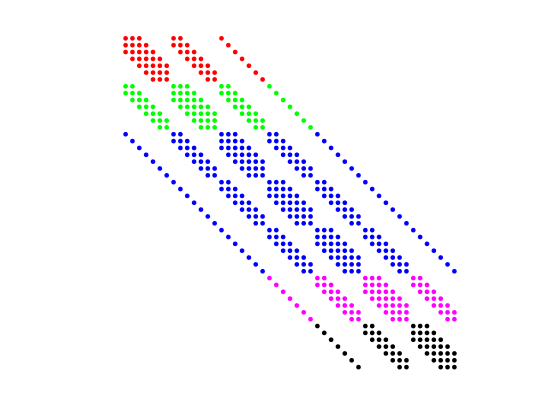
\includegraphics[width=0.35\linewidth]{./img/bhcolorus.pdf} }}%           
  \qquad
  \subfloat[\centering Block Indexing]
           {{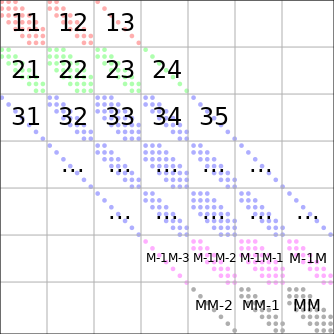
\includegraphics[width=0.35\linewidth]{./img/bhblocks.pdf} }}%
-  \caption{Biharmonic block structure. Each indexed block is computed separately and then concatenated together. Colour illustrates boundary sections of the biharmonic, with the central repeating section highlighted in blue. }%
  \label{fig:bh-block}%
\end{figure}
The second approach is to decompose the operator across the 13 diagonals and to separate them into non-repeating sectors. Each diagonal array is split into 3-5 sectors; each diagonal sector contains between 3-5 unique coefficients. Care must be taken to zero pad diagonals where necessary. The two boundary conditions (flexural and rotational spring stiffness) per edge of the plate mean 8 boundary stiffness coefficients (BSP), which impacts the repetition of diagonal patterns in the distribution of coefficients. Figure \ref{fig:biharm_zoom} illustrates the distribution of unique coefficients within the operator. As in Figure \ref{fig:bh-block}, Figure \ref{fig:biharm_zoom} shows a repeating central section but an overall lack of repeating diagonal patterns. 
\begin{figure}[H]
    \raggedleft
    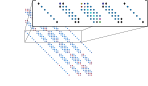
\includegraphics[width=0.7\linewidth]{./img/biharm_zoom.pdf}
    \caption{Detail of biharmonic block structures illustrating the impact of 8 BSP on internal symmetry.  Each marker/colour combination represents a unique coefficient.}
    \label{fig:biharm_zoom}
\end{figure}
The 13-point biharmonic stencil, as shown in Figure \ref{fig:PlateGhostFD}, only has 4 unique coefficients. In addition, two extra coefficients are required for the case of clamped and simply supported boundary conditions, implying that the biharmonic operator in those classical cases is composed of 6 unique coefficients. By contrast, the biharmonic operator with generalised elastic boundary conditions can contain up to 229 unique coefficients. As a result, each block or diagonal sector cannot be constructed through the repetition of a stencil pattern but must be declared explicitly. This lack of pattern repetition also impacts computational performance when constructing the operator. Since the biharmonic operator with generalised boundary condition provides very useful functionality in and of itself, the functionality to compute it is provided with an open interface as part of the library through the \texttt{bhmat} function \cite{MAGPIE_project_url}. The operator can then be used in further user-defined Finite Difference Time Domain schemes or if the users wish to take a more bespoke approach to eigenvalue/eigenvector calculation.


\subsection{Performance Across Implementations}
%One of the final goal of this project is to achieve real time computation of the biharmonic to use in sound-synthesizing modules. 
It was initially unclear which approach to composing the operator would yield the best performance. 
At the time of writing, the diagonal composition method was not yet finished with the Python implementation. 
\begin{figure}[H]
    \centering
    \includegraphics[width=0.9\linewidth]{./img/matlab_vs_python_eigs2.pdf}
    \caption{(a) Biharmonic operator computation performance comparison between diagonal formulation in MATLAB and block formulation in both MATLAB and python, (b) Eigensolver performance comparison between MATLAB and python for three different number of modes.}
    \label{fig:matlab_vs_python}
\end{figure}
Figure \ref{fig:matlab_vs_python} (a) compares the computing time necessary to build the biharmonic with increasing size, using a block structure, diagonal in MATLAB, and a block structure in Python. Each size of biharmonic was computed 10 times and the shortest time was recorded. The speed tests for the biharmonic operator computation in Figure \ref{fig:matlab_vs_python} show a clear performance superiority of the diagonal formulation over the block formulation in both MATLAB and Python languages. For the largest grid size ($3e^{5}$) tested in MATLAB, the diagonal method was forty times faster than the block method (results showing 0.2 seconds against 8 seconds respectively).
Given this result, it can be projected that a diagonal composition in Python will likely outperform the block composition method.

Figure \ref{fig:matlab_vs_python} (b) shows the MATLAB eigensolver outperforming the SciPy package's \texttt{eigs} function. It is possible that performance may improve when using a diagonal spare compression format. A non-intuitive result is that fewer modes can compute slower than a higher one. This is due to the search space being proportional to the number of eigenvalues requested, which may lead to eigenvalues being found faster for a higher number of modes. Interestingly enough, there is a similar phenomenon in MATLAB, and it will be of interest when optimizing the speed of MAGPIE in later stages of development. Performance benchmarking of alternative eigensolvers in Python is still ongoing.


\subsection{Case Study: Generalised Boundary Conditions}


This section presents a use-case of the MAGPIE library where a user wishes to explore the transition from a simply supported condition case to a clamped case by gradually increasing rotational spring stiffness across one edge of a plate and observing the effects on modal patterns and frequency response. The user first defines the plate material parameters, which are Young's modulus, density, Poisson number, and dimensions. These parameters compute the discrete biharmonic operator in a sparse matrix format. The biharmonic operator is then used as input for an eigensolver, which returns the eigenvalues and eigenvectors.

The user wishes to compare with Chladni patterns recorded during the course of experiments on a real plate. As such, the user chooses the 'Chladni' format option for plotting mode shapes. The `Chladni' option renders a top-down 2D visualisation of mode patterns where points at or near zero are highlighted. This allows the user to render Figure \ref{fig:bc_transitions}, which shows the effect of transition in the rotational stiffness.  From these plots obtained by MAGPIE, the user can illustrate how the mode shapes develop between simply supported and clamped cases. As expected, an increase in rotational stiffness increases modal frequency.
\begin{figure}[H]
    \centering
    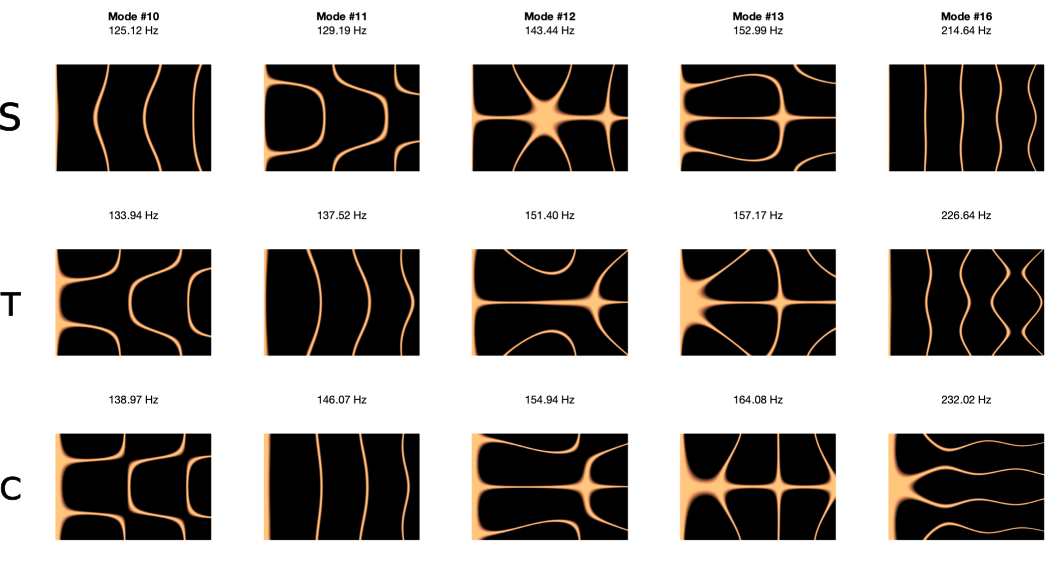
\includegraphics[width=0.75\linewidth]{./img/bc-transition.pdf}
    \caption{Simulated Chladni patterns of modes 10, 11, 12, 13, and 16, for a plate with free boundary conditions along all edges except the leftmost one. The last condition moves from simply supported (\textbf{S}) to a fully clamped cantilever case (\textbf{C}), with an intermediary step corresponding to a high rotation stiffness (\textbf{T}). The choice of specific modes is the result of an exploration using the Jupyter Notebook graphical interface depicted in Figure \ref{fig:magpie-ui} }
    \label{fig:bc_transitions}
\end{figure}
Secondly, the eigenvalues returned from the eigensolver are used to calculate modal frequencies. The user can then use the modal time integration functionality of MAGPIE using these modal frequencies, producing a simulated impulse response of the plate. The impulse response of the simulated is then used to create a series of FRF plots contrasting the transition between boundary conditions, as can be created as shown in \ref{fig:frf-bcs}.
\begin{figure}[H]
    \centering
    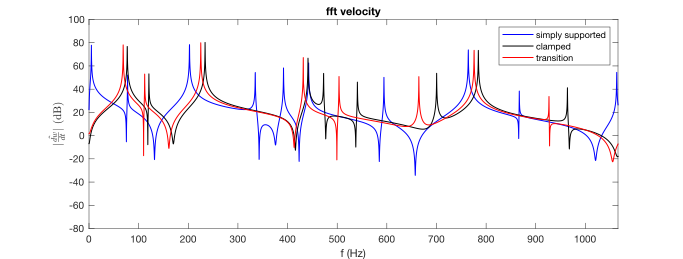
\includegraphics[width=0.8\linewidth]{./img/frf-bcs.pdf}
    \caption{FRF of impulse response from simulations of the same plate under different boundary conditions.}
    \label{fig:frf-bcs}
\end{figure}

\section{FINAL COMMENTS AND CONCLUSIONS}\label{sec:Conclusions}

% - The aim  for an open source library for modal analysis plate that is open source language agnostic.
%   - Project is open source available on the Nemus project's GitHub https://github.com/orgs/Nemus-Project/teams/magpie/repositories
%     - structured to expandable
%   - Identical functionality achieved across python and MATLAB  
%     - Mode freq and shape calculator
%     - Fast computation
%     - Chladni pattern and mode shape visualisation
%     - Time domain simulations
%   - an interface to the library through jupyter notebooks\\
  
The first version of an open source library for the modal analysis of plates was authored. The full code of the project is available on the Nemus project's GitHub \url{https://github.com/orgs/Nemus-Project/teams/magpie/repositories}. Care and attention has been given to the structure of the code, in order to make the library as modular and reusable to as wide an audience as possible. Central functionality was replicated in both MATLAB and Python, while taking care to accommodate for the conventions used by both programming languages. This functionality was namely the computation of the biharmonic operator in a sparse matrix format with generalized elastic boundary conditions, the computation the eigenfrequencies and eigenmodes, the visualisation the mode shapes. All of these data can then be used in time domain simulations. A graphical interface was designed using the Jupyter Notebooks platform by utilising the Python implementation of the library. \\  

% Going Forward:
% - implementations
%   - C / C++: 
%     - Going forward, the intention is for the library to be language agnostic. The next planned implementation would be in a C / C++ interface. 
%         - compilation as a library would allow for easy integration into other environments
%       - [MATLAB since 2021b](https://www.mathworks.com/help/matlab/call-c-library-functions.html)
%       - [Python as extension module](https://docs.python.org/3/extending/extending.html)
%       - [Web Assembly](https://webassembly.org/)
%     - inherent performance increase from a compiled language
% - interfaces
%   - MATLAB GUIDE
%   - Web: Ultimately it would be most beneficial to deploy MAGPIE on the client side in a web browser (making it even more accessible).
%     - via JavaScript
%     - Via Web Assembly
% - deployment
%   - as MATLAB add on
%   - via pip
%   - Public Server Service
%   - Progressive web app
% - Library Functionality
%   - - Nonlinear plate (I can write it tomorrow) check
%   - Orthotropic plate
%   - FASTER (Loop formalism , parallel diagonals)
%     - cases where the plate is symmetrical means that it can be optimised
%     - self contained sectors and blocks mean that concurrent computation is an option. Uncertain this will yield better performance as there are inherent overheads in multi-threading
%     - hardware testing:
%       - further extensive benchmarking across platforms and specifications to determine which algorithm to user.
%   - broader models in general (nonlinear bars and strings)
%   - Generalised Finite Difference Models
%     - fidimat check (kinda\\

Going forward, a broader set of models will be considered. The ongoing work concerns the Föppl–von Kármán model for nonlinear thin plates \cite{von_karman_probleme_1910}, which calls for the implementation of other operators in sparse matrix form. These operators are used in a variety of other models, such as the nonlinear bar and nonlinear string, which are other models that will be developed in MAGPIE. The orthotropic Kirchoff-Love plate is another direction to explore. The orthotropic model is the most interesting from a musical instrument manufacturing perspective as it would be a better approximation of wooden soundboard vibration. In combination with  generalised boundary conditions, an orthotropic model would allow for easier experimental comparison than the tools currently available. In terms of time efficiency, parallel computation of sectors and block have not yet been tested, but may yield better performances. The biharmonic operator computational performance could be further improved by separately considering specific cases such as square plate and symmetric boundary conditions where repeating coefficient patterns are more prevalent. Future development will include the implementation of a MATLAB package, a C / C++ library in addition to the expansion of the existing Jupyter Notebooks interface.
\noindent
